% !TEX root = saveliev_physics_general_course_2.tex
%!TEX TS-program = pdflatex
%!TEX encoding = UTF-8 Unicode


\chapter[THE CLASSICAL THEORY OF ELECTRICAL CONDUCTANCE\\ OF METALS]{THE CLASSICAL THEORY
OF\\ ELECTRICAL CONDUCTANCE OF\\ METALS}\label{chap:11}
\chaptermark{CLASSICAL THEORY OF ELECTRICAL CONDUCTANCE OF METALS}

\section{The Nature of Current Carriers in Metals}\label{sec:11_1}

A number of experiments were run to reveal the nature of the current carriers in metals.
Let us first of all note the experiment conducted in 1901 by the German physicist Carl Riecke (1845-1915).
He took three cylinders---two of copper and one of aluminium---with thoroughly polished ends.
After being weighed, the cylinders were put end to end in the sequence copper-aluminium-copper.
A current was passed in one direction through this composite conductor during a year.
During this time, a total charge of \SI{3.5e6}{\coulomb} passed through the cylinders.
Weighing showed that the passage of a current had no effect on the weight of the cylinders.
When the ends that had been in contact were studied under a microscope, no penetration of one metal into
another was detected.
The results of the experiment indicate that a charge is carried in metals not by atoms, but by particles encountered in all metals.
The electrons discovered by I. J. Thomson in 1897 could be such particles.

To identify the current carriers in metals with electrons, it was necessary to determine the sign and numerical value of the specific charge of the carriers.
Experiments run for this purpose were based on the following considerations.
If metals contain charged particles capable of moving, then upon the deceleration (braking) of a metal conductor these particles should continue to move by inertia for a certain time, as a result of which a current pulse will appear in the conductor, and a certain charge will be carried in it.

Assume that a conductor initially moves with the velocity $\vec{v}_0$ (\fig{11_1}).
We shall begin to decelerate it with the acceleration $\vec{a}$.
Continuing to move by inertia, the current carriers will acquire the acceleration $-\vec{a}$ relative to the conductor.
The same acceleration can be imparted to the carriers in a stationary conductor if an electric field of strength $\vec{E}=-m\vec{a}/e'$ is set up in it, \ie, the potential difference,
\begin{equation*}
    \varphi_1 - \varphi_2 = \int_1^2 \vec{E} \ccdot \derivec{l} = -\int_1^2 \frac{m \vec{a}}{e'} \ccdot \derivec{l} = - \frac{mal}{e'},
\end{equation*}

\noindent
is applied to the ends of the conductor ($m$ and $e'$ are the mass and the charge of a current carrier, $l$ is the length of a conductor).
In this case, the current $I = (\varphi_1 - \varphi_2)/R$, where $R$ is the resistance of the conductor, will flow through it ($I$ is considered to be positive if the current flows in the direction of motion of the conductor).
Hence, the following charge will pass through each cross section of the conductor during the time $\deriv{t}$:
\begin{equation*}
    \deriv{q} = I\, \deriv{t} = - \frac{mal}{e'R}\, \deriv{t} = - \frac{ml}{e'R}\, \deriv{v}.
\end{equation*}

\noindent
The charge passing during the entire time of deceleration is
\begin{equation}\label{eq:11_1}
    q = \int_1^2 \deriv{q} = - \int_{v_0}^0 \frac{ml}{e'R}\, \deriv{v} = \frac{m}{e'} \frac{lv_0}{R}
\end{equation}

\noindent
(the charge is positive if it is carried in the direction of motion of the conductor).

\begin{figure}[t]
	\begin{center}
		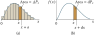
\includegraphics[scale=1]{figures/ch_11/fig_11_1.pdf}
		\caption[]{}
		\label{fig:11_1}
	\end{center}
	\vspace{-0.8cm}
\end{figure}

Thus, by measuring $l$, $v_0$, and $R$, and also the charge $q$ flowing through the circuit when the conductor is decelerated, we can find the specific charge of the carriers.
The direction of the current pulse will indicate the sign of the carriers.

The first experiment with conductors moving with acceleration was run in 1913 by the Soviet physicists Leonid Mandelshtam (1879-1944) and Nikolai Papaleksi (1880-1947).
They made a wire coil perform rapid torsional oscillations about its axis. A telephone was connected to the ends of the coil, and the sound due to the current pulses was heard in it.

A quantitative result was obtained by the American physicists R. Tolman and T. Stewart in 1916. A coil of a wire \SI{500}{\metre} long was made to rotate with a linear velocity of the turns of \SI{300}{\metre\per\second}.
The coil was then sharply braked, and a ballistic galvanometer was used to measure the charge flowing in the circuit during the braking time.
The value of the specific charge of the carriers calculated by \eqn{11_1} was obtained very close to $e/m$ for electrons.
It was, thus, proved experimentally that electrons are the current carriers in metals.

A current can be produced in metals by an extremely small potential difference.
This gives us the grounds to consider that the current carriers---electrons---move without virtually any hindrance in a metal.
The result of Tolman's and Stewart's experiment lead to the same conclusion.

The existence of free electrons in metals can be explained by the fact that when a crystal lattice is formed, the most weakly bound (valence) electrons detach themselves from the atoms of the metal.
They become the ``collective'' property of the entire piece of metal.
If one electron becomes detached from every atom, then the concentration of the free electrons (\ie, their number $n$ in a unit volume) will equal the number of atoms in a unit volume.
The latter number is $(\delta/M)\ab{N}{A}$, where $\delta$ is the density of the metal, $M$ is the mass of a mole, $\ab{N}{A}$ is Avogadro's constant.
The values of $\delta/M$ for metals range from \SI{2e4}{\mole\per\metre\cubed} (for potassium) to \SI{2e5}{\mole\per\metre\cubed} (for beryllium).
Hence, we get values of the following order for the concentration of the free electrons (or conduction electrons, as they are also called):
\begin{equation}\label{eq:11_2}
    n = \text{\SIrange{e28}{e29}{\per\metre\cubed}} \parenthesis{\text{\SIrange{e22}{e23}{\per\centi\metre\cubed}}}.
\end{equation}

\section{The Elementary Classical Theory of Metals}\label{sec:11_2}

Proceeding from the notions of free electrons, the German physicist Paul Drude (1863-1906) created the classical theory of metals that was later improved by H. Lorentz.
Drude assumed that the conduction electrons in a metal behave like the molecules of an ideal gas.
In the intervals between collisions, they move absolutely freely, covering on an average a certain path $l$.
True, unlike the molecules of a gas whose free path is determined by collisions of the molecules with one another, the electrons collide chiefly not with one another, but with the ions forming the crystal lattice of the metal.
These collisions result in the establishment of thermal equilibrium between the electron gas and the crystal lattice.

Assuming that the results of the kinetic theory of gases may be extended to an electron gas, we can use the following formula to assess the average velocity of thermal motion of the electrons:
\begin{equation}\label{eq:11_3}
    \average{v} = \parenthesis{\frac{8kT}{\pi m}}^{1/2}
\end{equation}

\noindent
[see Eq. (11.65) of Vol. I].
Calculations by this equation for room temperature (about \SI{300}{\kelvin}) give the following result:
\begin{equation*}
    \average{v} = \parenthesis{\frac{8 \times \num{1.38e-23} \times 300}{ 3.14 \times \num{0.91e-30} }}^{1/2} \approx \SI{e5}{\metre\per\second}.
\end{equation*}

When a field is switched on, the ordered motion of the electrons with a certain average velocity $\average{u}$ is superposed onto the chaotic thermal motion occurring with the velocity $\average{v}$.
It is simple to assess the value of $\average{u}$ by the equation
\begin{equation}\label{eq:11_4}
    j = ne\average{u}
\end{equation}

\noindent
[see \eqn{5_23}].
The maximum current density for copper wires allowed by the relevant specifications is about \SI{e7}{\ampere\per\metre\squared} (\SI{10}{\ampere\per\milli\metre\squared}).
Taking the value of \SI{e29}{\per\metre\cubed} for $n$, we get
\begin{equation*}
    \average{u} = \frac{j}{en} \approx \frac{\num{e7}}{\num{1.6e-19} \times \num{e29}} \approx \SI{e-3}{\metre\per\second}.
\end{equation*}

\noindent
Thus, even at very high current densities, the average velocity of ordered motion of the charges $\average{u}$ is about $1/\num{e8}$ of the average velocity of thermal motion $\average{v}$.
Therefore, in calculations, the magnitude of the resultant velocity $|\vec{v}+\vec{u}|$ may be replaced with that of the velocity of thermal motion $|\vec{v}|$.

Let us find the change in the mean value of the kinetic energy of the electrons produced by a field.
The mean square of the resultant velocity is
\begin{equation}\label{eq:11_5}
    \average{(\vec{v}+\vec{u})^2} = \average{\vec{v}^2 + 2\vecdot{v}{u} + \vec{u}^2} = \average{\vec{v^2}} + 2 \average{\vecdot{v}{u}} + \average{\vec{u}^2}.
\end{equation}

\noindent
The two events consisting in that the velocity of thermal motion of the electrons will take on the value $\vec{v}$, while the velocity of ordered motion---the value $\vec{u}$, are statistically independent.
Therefore, according to the theorem on the multiplication of probabilities [see Eq. (11.4) of Vol. I], we have $\average{\vecdot{v}{u}} = \average{\vec{v}}\ccdot\average{\vec{u}}$.
But $\average{\vec{v}}$ equals zero, so that the second addend in \eqn{11_5} vanishes, and it acquires the form
\begin{equation*}
    \average{(\vec{v}+\vec{u})^2} = \average{\vec{v^2}} + \average{\vec{u}^2}.
\end{equation*}

\noindent
Hence, it follows that the ordered motion increases the kinetic energy of the electrons on an average by
\begin{equation}\label{eq:11_6}
    \average{\Delta{\ab{\varepsilon}{k}}} = \frac{m\average{u^2}}{2}.
\end{equation}

\textbf{Ohm's Law.} Drude considered that when an electron collides with an ion of the crystal lattice, the additional energy \eqref{eq:11_6} acquired by the electron is transmitted to the ion and, consequently, the velocity $u$ as a result of the collision vanishes.
Let us assume that the field accelerating the electrons is homogeneous.
Hence, under the action of the field, the electron receives a constant acceleration equal to $eE/m$, and toward the end of its path the velocity of ordered motion will reach, on an average, the value
\begin{equation}\label{eq:11_7}
    \ab{u}{max} = \frac{eE}{m} \tau,
\end{equation}

\noindent
where $\tau$ is the average time elapsing between two consecutive collisions of the electron with ions of the lattice.

Drude did not take into consideration the distribution of the electrons by velocities and ascribed the same value of the velocity $v$ to all the electrons.
In this approximation
\begin{equation*}
    \tau = \frac{l}{v}
\end{equation*}

\noindent
(we remind our reader that $|\vec{v}+\vec{u}|$ virtually equals $|\vec{v}|$).
Using this value of $\tau$ in \eqn{11_7}, we get
\begin{equation}\label{eq:11_8}
    \ab{u}{max} = \frac{eEl}{mv}.
\end{equation}

\noindent
The velocity $u$ changes linearly during the time it takes to cover the path $l$.
Therefore, its average value over the path equals half the maximum value:
\begin{equation*}
    \average{u} = \frac{1}{2} \ab{u}{max} = \frac{eEl}{2mv}.
\end{equation*}

\noindent
Introducing this equation into \eqn{11_4}, we get
\begin{equation*}
    j = \frac{ne^2l}{2mv} E.
\end{equation*}

The current density is found to be proportional to the field strength.
We have, thus, arrived at Ohm's law.
According to \eqn{5_22}, the constant of proportionality between $j$ and $E$ is the conductivity
\begin{equation}\label{eq:11_9}
    \sigma = \frac{ne^2l}{2mv}.
\end{equation}

\noindent
If the electrons did not collide with the ions of the lattice, their free path and, consequently, the conductivity of the metal would be infinitely great.
Thus, \textit{according to the classical notions, the electrical resistance of metals is due to the collisions of their free electrons with the ions at the crystal lattice points of the metal}.

\textbf{The Joule-Lenz Law.} By the end of its free path, an electron acquires additional kinetic energy whose average value is
\begin{equation}\label{eq:11_10}
    \average{\Delta{\ab{\varepsilon}{k}}} = \frac{m \ab{u}{max}^2}{2} = \frac{e^2l^2}{2mv} E^2
\end{equation}

\noindent
[see \eqns{11_6}{11_8}].
Upon colliding with an ion, the electron, according to the assumption, completely transfers the additional energy it has acquired to the crystal lattice.
The energy given up to the lattice goes to increase the internal energy of the metal, which manifests itself in its becoming heated.

Every electron experiences on an average $1/\tau=v/l$ collisions a second, communicating each time the energy expressed by \eqn{11_10} to the lattice.
Hence, the following amount of heat should be liberated in unit volume per unit time:
\begin{equation*}
    \ab{Q}{u} = n \frac{1}{\tau} \average{\Delta{\ab{\varepsilon}{k}}} = \frac{ne^2l}{2mv} E^2
\end{equation*}

\noindent
($n$ is the number of conduction electrons per unit volume).

The quantity $\ab{Q}{u}$ is the unit thermal power of a current (see \sect{5_8}).
The factor of $E^2$ coincides with the value given by \eqn{11_9} for $\sigma$.
Passing over in the expression $\sigma E^2$ from $\sigma$ and $E$ to $\rho$ and $j$, we arrive at the formula $\ab{Q}{u}=\rho j^2$ expressing the Joule-Lenz law [see \eqn{5_39}].

\textbf{The Wiedemann-Franz Law.} It is known from experiments that in addition to their high electrical conductivity, metals are distinguished by a high thermal conductivity.
The German physicists G. Wiedemann and R. Franz discovered an empirical law according to which the ratio of the thermal conductivity $\varkappa$ to the electrical conductivity $\sigma$ is about the same for all metals and changes in proportion to the absolute temperature.
For example, for aluminium at room temperature, this ratio is \SI{5.8e-6}{\joule\ohm\per\second\per\kelvin}, for copper it is \SI{6.4e-6}{\joule\ohm\per\siemens\per\kelvin}, and for lead it is \SI{7.0e-6}{\joule\ohm\per\second\per\kelvin}.

Non-metallic crystals are also capable of conducting heat.
The thermal conductivity of metals, however, considerably exceeds that of dielectrics.
It thus follows, that the free electrons instead of the crystal lattice are responsible for the transfer of heat in metals.
Considering these electrons as a monatomic gas, we can adopt an expression from the kinetic theory of gases for the thermal conductivity:
\begin{equation}\label{eq:11_11}
    \varkappa = \frac{1}{3} n m v l c_V
\end{equation}

\noindent
[see Eq. (16.26) of Vol. I; the density $\rho$ has been replaced with the product $nm$, and $\average{v}$ with $v$].
The specific heat capacity of a monatomic gas is $c_V = 3R/(2M) = 3k/(2m)$.
Using this value in \eqn{11_11}, we obtain
\begin{equation*}
    \varkappa = \frac{1}{2} n k v l.
\end{equation*}

Dividing $\varkappa$ by \eqn{11_9} for $\sigma$ and then substituting $3k/(2T)$ for $mv^2/2$, we arrive at the expression
\begin{equation}\label{eq:11_12}
    \frac{\varkappa}{\sigma} = \frac{k m v^2}{e^2} = 3 \parenthesis{\frac{k}{e}}^2 T.
\end{equation}

\noindent
that expresses the Wiedemann-Franz law.

Introduction of the numerical values of $k$ and $e$ into \eqn{11_12} yields
\begin{equation*}
    \frac{\varkappa}{\sigma} = \num{2.23e-8}\, T.
\end{equation*}

\noindent
When $T = \SI{300}{\kelvin}$, we get the value \SI{3.7e-6}{\joule\ohm\per\second\per\kelvin} for $\varkappa/\sigma$, which agrees quite well with experimental data (see the values of $\varkappa/\sigma$ given above for aluminium, copper, and lead).
It was later established, however, that such a good coincidence is accidental, because when H. Lorentz performed the calculations more accurately, taking
into account the distribution of the electrons by velocities, the value of $2(k/e)^2 T$ was obtained for the ratio $\varkappa/\sigma$, and it does not agree so well with the data of experiments.

Thus, the classical theory was able to explain Ohm's and the Joule-Lenz laws, and also gave a qualitative explanation of the Wiedemann-Franz law.
At the same time, this theory encountered quite appreciable difficulties.
They include two basic ones.
It can be seen from \eqn{11_9} that the resistance of metals (\ie, the quantity that is the reciprocal of $\sigma$) must increase as the square root of $T$.
Indeed, we have no grounds to assume that the quantities $n$ and $l$ depend on the temperature.
The velocity of thermal motion, on the other hand, is proportional to the square root of $T$.
This theoretical conclusion contradicts experimental data according to which the electrical resistance of metals grows in proportion to the first power of $T$, \ie, more rapidly than $T^{1/2}$ [see expression \eqref{eq:5_24}].

The second difficulty of the classical theory is that an electron gas must have a molar heat capacity equal to $(3/2)R$.
Adding this quantity to the heat capacity of the lattice, which is $3R$ [see Eq. (13.1) of Vol. I], we get the value of $(9/2)R$ for the molar heat capacity of a metal.
Thus, in accordance with the classical electron theory, the molar heat capacity of metals ought to be $1.5$ times higher than that of dielectrics.
Actually, however, the heat capacity of metals does not differ appreciably from that of non-metallic crystals.
Only the quantum theory of metals was able to explain this discrepancy.

\section{The Hall Effect}\label{sec:11_3}

If a metal plate through which a steady electric current is flowing is placed in a magnetic field perpendicular to it, then a potential difference of $\ab{U}{H} = \varphi_1 - \varphi_2$ (\fig{11_2}) is set up between the plate faces parallel to the directions of the current and field.
This phenomenon was discovered by the American physicist E. Hall in 1879 and is called the \textbf{Hall effect} or the \textbf{galvanomagnetic effect}.

\begin{figure}[t]
	\begin{minipage}[t]{0.48\linewidth}
		\begin{center}
			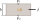
\includegraphics[scale=1]{figures/ch_11/fig_11_2.pdf}
			\caption[]{}
			\label{fig:11_2}
		\end{center}
	\end{minipage}
	\hfill{ }%space{-0.05cm}
	\begin{minipage}[t]{0.48\linewidth}
		\begin{center}
			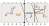
\includegraphics[scale=1]{figures/ch_11/fig_11_3.pdf}
			\caption[]{}
			\label{fig:11_3}
		\end{center}
	\end{minipage}
\vspace{-0.4cm}
\end{figure}

The Hall potential difference is determined by the expression
\begin{equation}\label{eq:11_13}
    \ab{U}{H} = \ab{R}{H} b j B.
\end{equation}

\noindent
Here, $b$ is the width of the plate, $I$ the current density, $B$ the magnetic induction of the field and $ab{R}{H}$ is a constant of proportionality known as the \textbf{Hall coefficient}.

The Hall effect is easily explained by the electron theory.
In the absence of a magnetic field, the current in the plate is due to the electric field $\vec{E}_0$ (\fig{11_3}).
The equipotential surfaces of this field form a system of planes perpendicular to the vector $\vec{E}_0$.
Two of them are shown in the figure by solid straight lines.
The potential at all the points of each surface and, consequently, at points $1$ and $2$ too is the same.
The current carriers---electrons---have a negative charge, therefore, the velocity of their ordered motion $\vec{u}$ is directed oppositely to the current density vector $\vec{j}$.

When the magnetic field is switched on, each carrier experiences the magnetic force $\vec{F}$ directed along side $b$ of the plate and having a magnitude of
\begin{equation}\label{eq:11_14}
    F = euB.
\end{equation}

\noindent
As a result, the electrons acquire a velocity component directed toward the upper (in the figure) face of the plate.
A surplus of negative charges is formed at this face and, accordingly, a surplus of positive charges at the lower face.
Consequently, an additional transverse electric field $\vec{E}_B$ is produced.
When the strength of this field reaches a value such that its action on the charges balances the force given by \eqn{11_14}, a stationary distribution of the charges in a transverse direction will set in.
The corresponding value of $E_B$ is determined by the condition $eE_B = euB$.
Hence,
\begin{equation*}
    E_B = uB.
\end{equation*}

The field $\vec{E}_B$ adds to the field $\vec{E}_0$ to form the resultant field $\vec{E}$.
The equipotential surfaces are perpendicular to the field strength vector.
Consequently, they will turn and occupy the position shown by the dash line in \fig{11_3}.
Points $1$ and $2$ which were formerly on the same equipotential surface now have different potentials.
To find the voltage appearing between these points, the distance $b$ between them must be multiplied by the strength $E_B$:
\begin{equation*}
    \ab{U}{H} = b E_B = b u B.
\end{equation*}

\noindent
Let us express $u$ through $j$, $n$, and $e$ in accordance with the equation $j = neu$.
The result is
\begin{equation}\label{eq:11_15}
    \ab{U}{H} = \frac{1}{ne} b j B.
\end{equation}

\noindent
Equations \eqref{eq:11_13} and \eqref{eq:11_15} coincide if we assume that
\begin{equation}\label{eq:11_16}
    \ab{R}{H} = \frac{1}{ne}.
\end{equation}

Inspection of \eqn{11_16} shows that by measuring the Hall coefficient, we can find the concentration of the current carriers in a given metal (\ie, the number of carriers per unit volume).

An important characteristic of a substance is the mobility of the current carriers in it.
By the mobility of the current carriers is meant the average velocity acquired by the carriers at unit electric field strength.
If the carriers acquire the velocity $u$ in a field of strength $E$, then their mobility $u_0$ is
\begin{equation}\label{eq:11_17}
    u_0 = \frac{u}{E}.
\end{equation}

\noindent
The mobility can be related to the conductivity $\sigma$ and to the carrier concentration $n$.
For this purpose, let us divide the equation $j=neu$ by the field strength $E$.
Taking into account that $j/E=\sigma$ and $u/E=u_0$, we get
\begin{equation}\label{eq:11_18}
    \sigma = ne u_0.
\end{equation}

Having measured the Hall coefficient $\ab{R}{H}$ and the conductivity $\sigma$, we can use \eqns{11_16}{11_18} to find the concentration and
mobility of the current carriers in the relevant specimen.

The Hall effect is observed not only in metals, but also in semiconductors.
The sign of the effect can be used to see whether a semiconductor belongs to the n- or p-type\footnote{In n-type semiconductors, the current carriers are negative, and in p-type ones they are positive (see Vol. III).}.
Figure \ref{fig:11_4} compares the Hall effect for specimens with positive and negative carriers.
The direction of the magnetic force is reversed both when the direction of motion of the charge changes and when its sign is reversed.
Hence, when the current and field have the same direction, the magnetic force exerted on positive and negative carriers has the same direction.
Therefore, with positive carriers, the potential of the upper (in the figure) face is higher than that of the lower one, and with negative carriers the potential is lower.
We can thus establish the sign of the current carriers after determining that of the Hall potential difference.

\begin{figure}[t]
	\begin{center}
		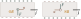
\includegraphics[scale=1]{figures/ch_11/fig_11_4.pdf}
		\caption[]{}
		\label{fig:11_4}
	\end{center}
	\vspace{-0.8cm}
\end{figure}

It is of interest to note that in some metals the sign of $\ab{U}{H}$ corresponds to positive current carriers.
This anomaly is explained by the quantum theory.
